
\chapter{Context}

\begin{figure}[htb]
\begin{center}
\leavevmode
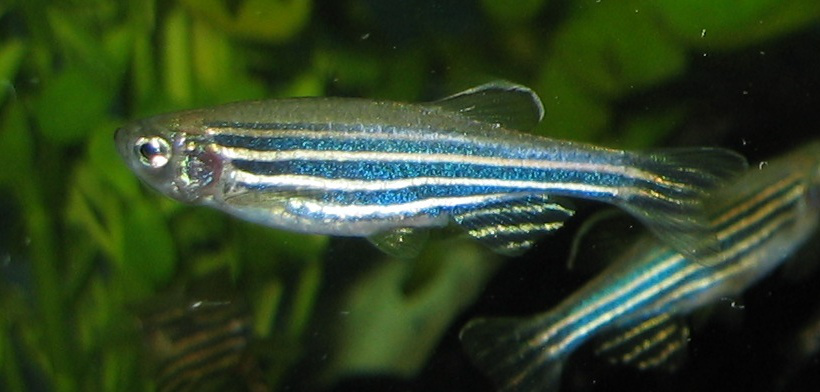
\includegraphics[width=0.99\textwidth]{pictures/zebrafishPic}
\end{center}
\caption{Mature zebra fish: approximatively 2.5cm long (source: \href{http://en.wikipedia.org/wiki/File:Zebrafisch.jpg}{Wikipedia})}
\label{fig:ZebraPic}
\end{figure}

\section{Systems Biology}

With the completion of the genome projects~\cite{}, the stage is now set for a
more complete understanding of how animals are created. Biologists now have
access to the complete sequence of DNA that encodes the blueprint of life for
many animals including human, mouse, zebrafish, and fruit
fly~\cite{[2][3][4][5]} \TODO{refe?}The challenge is now understanding how this
code functions. The problem however is that the only thing that biologists can
currently reliably predict from the genomic code is which parts can be
transcribed and translated into protein. Biologists cannot accurately predict
when and where a protein will be expressed, how a protein will
function once it is created, and the interaction between expressed proteins that
allow them to form functional genetic circuits. Thus, although the genome
projects have given us the complete code for constructing many organisms, the
only part of the code biologists can currently read is the parts list. The
challenge is understanding how all these parts fit together to form molecular
circuits, how these circuits process information to regulate the behavior of
cells, and how the behavior of cells is orchestrated to generate functional form
as in \emph{embryogenesis}. This post-genomic endeavor has come to be called
\emph{systems biology}.\\

Although systems biology grew out of the “-omics” field which made heavy use of 
in vitro biochemical approaches (e.g. sequencing, microarrays, and proteomics),
\textit{in-vivo} imaging is becoming an increasingly powerful tool for
systems biology. \textit{In-vivo} imaging is advantageous over
biochemical approaches for doing systems biology:

\begin{itemize}
 \item Biological circuits function at the single cell level. Microscopic
imaging easily achieves this resolution while in-vitro techniques do not.
 \item Biological circuits function over time. With imaging, different
components of a biological circuit can be labeled using different colors of
fluorescent proteins and the dynamics of the circuit monitored non-invasively
with time-lapse fluorescent imaging as the circuit functions in an intact
system. In vitro biochemical approaches typically require the tissue to
be destroyed in order to be assayed which precludes longitudinal analysis.
 \item the quantitative amounts of components in a biological circuit are
important for its function. Fluorescent imaging can accurately quantitate the
levels of molecular components even at the protein level through the use of
fluorescent protein (e.g. GFP) fusions. Omic approaches are typically less
quantitative and focus at the DNA or RNA level which is less relevant.
 \item the anatomical context of biological circuits is essential for
determining their function; the use of spatial cues to generate different cell
types in different places is a fundamental aspect of development. In vivo
imaging can capture data from intact animals preserving its anatomical context.
In vitro approaches typically grind up the tissue to assay it, thus destroying
its anatomy.
\end{itemize}

%%%%%%%%%%%%%%%%%%%%%%%%%%%%%%%%%%%%%%%%%%%%%%%%%%%%%%%%%%%%%%%%%%%%%%%%%%%%%%%
%%%%%%%%%%%%%%%%%%%%%%%%%%%%%%%%%%%%%%%%%%%%%%%%%%%%%%%%%%%%%%%%%%%%%%%%%%%%%%%
%%%%%%%%%%%%%%%%%%%%%%%%%%%%%%%%%%%%%%%%%%%%%%%%%%%%%%%%%%%%%%%%%%%%%%%%%%%%%%%

\section{Zebrafish: one sytem of high interest for Systems-Biology}

Zebrafish (Danio rerio) is a small, freshwater, tropical fish commonly available
in pet stores (see figure~\ref{}). It has become a popular model system for the
study of genetics and development in the last 2 decades and there are now
many labs worldwide that study it. There have been several
large-scale mutagenesis screens caried out in zebrafish and its genome has been
largely sequenced. Zebrafish has the advantages of fruit fly in that it
is amenable to forward genetic screens, but unlike fruit fly, zebrafish is a
vertebrate so is much more relevant to humans. Another huge advantage
of zebrafish is its suitability for imaging. Zebrafish embryos are transparent,
small, develop freely outside their mother, and develop directly from egg to
adult without any larval stages. This means that a zebrafish egg can be placed
under a microscope and continuously imaged throughout embryogenesis. This would
be impossible with a mouse which develop inside its mother, with a frog
(Xenopus) egg which is opaque, or with a fruit fly (Drosophila) which has
several larval/pupal stages and is opaque.

%%%%%%%%%%%%%%%%%%%%%%%%%%%%%%%%%%%%%%%%%%%%%%%%%%%%%%%%%%%%%%%%%%%%%%%%%%%%%%%
%%%%%%%%%%%%%%%%%%%%%%%%%%%%%%%%%%%%%%%%%%%%%%%%%%%%%%%%%%%%%%%%%%%%%%%%%%%%%%%
%%%%%%%%%%%%%%%%%%%%%%%%%%%%%%%%%%%%%%%%%%%%%%%%%%%%%%%%%%%%%%%%%%%%%%%%%%%%%%%

\section{In-toto imaging: one technique of interest for Systems-Biology}

The goal of in toto imaging is to image and track every single cell in a
developing tissue, organ, or eventually
whole embryo~\cite{megason2003digitizing}. This technique will provide
significant outcomes in a complete understanding of the cellular basis of
development through the construction of complete lineage trees\footnote{First
results on early zebrafish embryo~\cite{SCIENCE-PAPER} show the immense impact
on the scientific community of such a technique.}. There are several steps to in
toto imaging.\\

The embryos must first be labeled with “segmentation markers” which allow all
the cells to be segmented. Additionally embryos can be labeled with additional
markers to reveal RNA or protein expression. The next step is to acquire 3D+t
image sets using confocal or 2-photon fluorescent microscopy. And the final step
is processing the often very large image sets to segment out all the cell
trajectories and to extract quantitative, cell-centric data.

\subsection{Embryo Labeling}

The living embryos must be labeled with fluorescent markers and imaged with
time-lapse technique. Biologists must use vital labels such as Green
Fluorescent Protein (GFP), or other available Fluorescence Proteins (FPs) across
the visible spectrum. Since FPs are proteins rather than organically synthesized
small molecule dyes, FPs can be endogenously expressed by transgenic organisms
and are open to all the power of genetic engineering.\\

There are 2 basic uses of markers for in toto imaging: segmentation and
expression.
\begin{itemize}
 \item Segmentation markers allow the cells to be segmented in space,
across time, and across cell-division. Biologists, at the Megason Lab, typically
use a histone-FP of one color (e.g. histone-cerulean) and a membrane-localized
FP of another color (e.g. membrane-mCherry). This combination would generate
embryos in which every nuclei is green and all the cell membranes are red~(see
figure~\ref{}).
 \item Expression markers refer to whatever else is being marked such that it
can be digitized with in toto imaging. For example, transgenic fish can be made
that express a fluorescent protein wherever some gene is normally expressed
during development.
\end{itemize}

%%%%%%%%%%%%%%%%%%%%%%%%%%%%%%%%%%%%%%%%%%%%%%%%%%%%%%%%%%%%%%%%%%%%%%%%%%%%%%%
%%%%%%%%%%%%%%%%%%%%%%%%%%%%%%%%%%%%%%%%%%%%%%%%%%%%%%%%%%%%%%%%%%%%%%%%%%%%%%%
%%%%%%%%%%%%%%%%%%%%%%%%%%%%%%%%%%%%%%%%%%%%%%%%%%%%%%%%%%%%%%%%%%%%%%%%%%%%%%%

\subsection{Image acquisition}

\subsubsection{Requirements}

In toto imaging tracks cells during development only by the correspondence of
cells from frame to frame. This is quite different than traditional fate mapping
in developmental biology where only a small subset of cells is labeled at one
stage of development and the location of their progeny is observed at a
later stage. In toto imaging thus requires images that have high enough
resolution in space to resolve all the cells (this requires $\approx
1 \mu$m resolution) and high enough resolution in time to not lose track of
moving and dividing cells (this requires $\approx 2$ min time resolution). In
addition to high resolution, in toto imaging also requires complete coverage.
All the cells of interest must be continuously imaged in order to be tracked; if
cells leave the field of view then their lineage cannot be completely tracked.

\subsubsection{Equipment}

Achieving both high spatial and temporal resolution as well as complete coverage
can be achieved through the use of time-lapse confocal or 2-photon microscopy.
Confocal microscopy~(see figure~\ref{fig:ConfocalPrinciple}) uses a pinhole to
eliminate out of focus light whereas 2-photon microscopy only excites
fluorescence in the focal plane.

Thus both techniques allow thin (1$\mu$m) optical sections of fluorescent
samples to be captured. By imaging at a series of focal planes, stacks of
optical sections can be captured to generate a volumetric image and this can be
repeated over time to generate 3D+t images. The axial (z) resolution with these
techniques is typically around 5-fold less than the planar (xy) resolution so
the volumetric images are anisotropic. Confocal imaging provides 2-fold higer
resolution than 2-photon imaging but has a depth penetration limit of  150 um.
2-photon imaging can image all the way through a zebrafish embryo and has
reduced phototoxicity to the embryo and photobleaching of the fluorescent
labels.\\

Both acquisition techniques have been assembled in the Megasaon Lab from a
Zeiss 710 NLO (figure~\ref{fig:MicMegason}).


\begin{figure}[htb]
\begin{center}
\leavevmode
 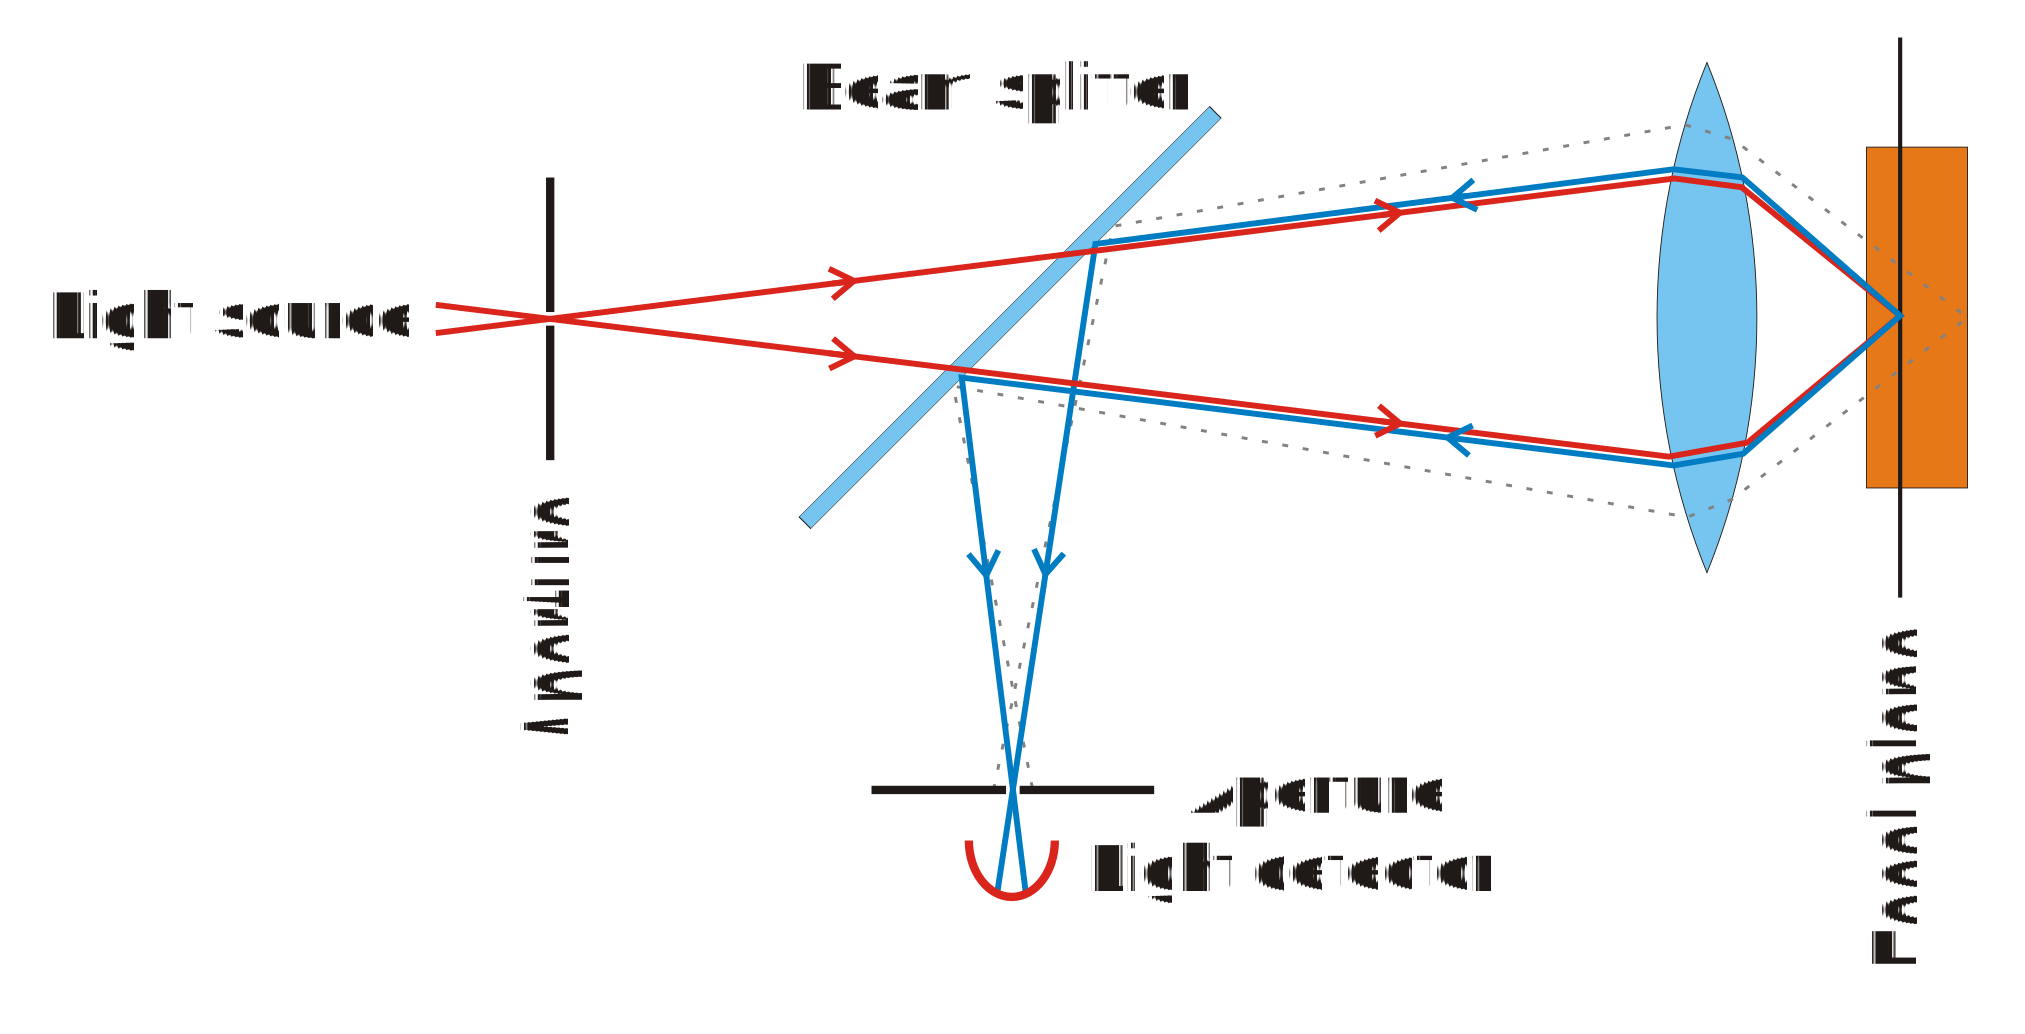
\includegraphics[width=0.95\textwidth]{pictures/ConfocalPrinciple}
\end{center}
\caption{Confocal microscope principle
(source:\href{http://en.wikipedia.org/wiki/File:Confocalprinciple.svg}{Wikipedia
})}
\label{fig:ConfocalPrinciple}
\end{figure}

\begin{figure}[htb]
\begin{center}
\leavevmode
 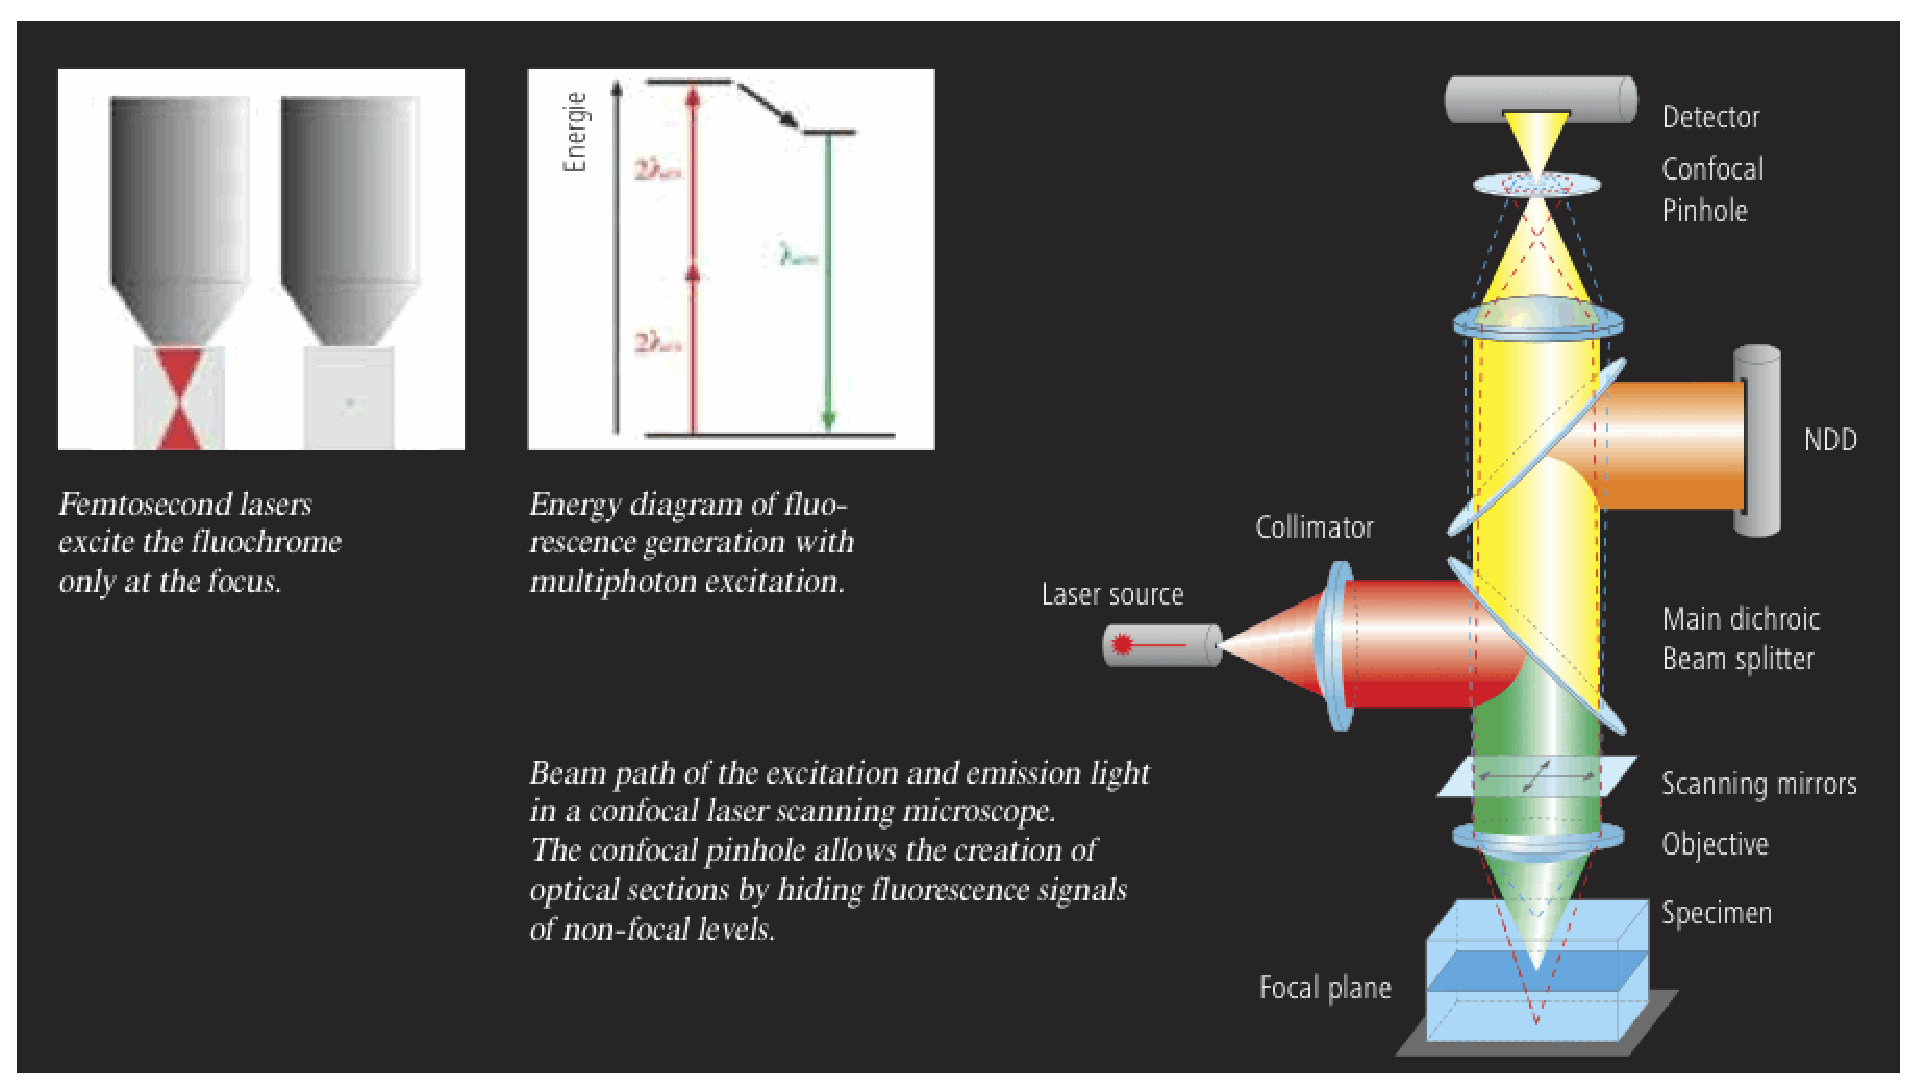
\includegraphics[width=0.95\textwidth]{pictures/ConfocalZeissPrinciple}
\end{center}
\caption{2-photon confocal microscope principle (Zeiss documentation)}
\label{fig:Confocal2photonsPrinciple}
\end{figure}

\begin{figure}[htb]
\begin{center}
\leavevmode
 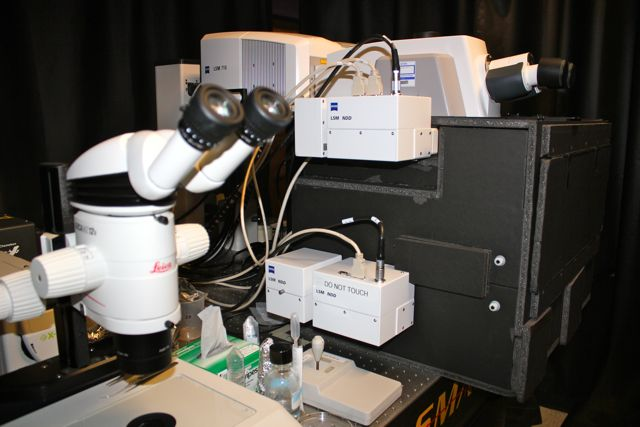
\includegraphics[width=0.95\textwidth]{pictures/PICmicroscope}
\end{center}
\caption{2-photon confocal microscope Zeiss 710 NLO in service in the Megason
Lab}
\label{fig:MicMegason}
\end{figure}

%%%%%%%%%%%%%%%%%%%%%%%%%%%%%%%%%%%%%%%%%%%%%%%%%%%%%%%%%%%%%%%%%%%%%%%%%%%%%%%
%%%%%%%%%%%%%%%%%%%%%%%%%%%%%%%%%%%%%%%%%%%%%%%%%%%%%%%%%%%%%%%%%%%%%%%%%%%%%%%
%%%%%%%%%%%%%%%%%%%%%%%%%%%%%%%%%%%%%%%%%%%%%%%%%%%%%%%%%%%%%%%%%%%%%%%%%%%%%%%

\subsection{Image Processing}

After the embryos have been labelled and imaged, the final challenge of in toto
imaging is image processing. The goal of image processing is to track all the
cell movements and divisions to generate cell lineage trees, to define the
boundaries of all cells and their compartments (nucleus, cytoplasm, membrane,
extracellular space), and to quantize the level of fluorescence within each
cell and subcellular compartment.\\

In order to process all the acquired data, an image processing team of
is working on the next platform of microscopy images analysis: {\gofigure}.
Their goal is to create a very accessible "cross-platform"\footnote{In
computing, cross-platform, or multi-platform, is
an attribute conferred to computer software or computing methods and concepts
that are implemented and inter-operate on multiple operating systems and
hardware.}, "open-source"\footnote{of or
relating to or being computer software for which
the source code is freely available, but which use may be restricted by a
license.}, freely distributed, application with a high quality code, for
biologists to process their data and for computer scientists and image
processing specialists the opportunity to promote their methods.

%%%%%%%%%%%%%%%%%%%%%%%%%%%%%%%%%%%%%%%%%%%%%%%%%%%%%%%%%%%%%%%%%%%%%%%%%%%%%%%
%%%%%%%%%%%%%%%%%%%%%%%%%%%%%%%%%%%%%%%%%%%%%%%%%%%%%%%%%%%%%%%%%%%%%%%%%%%%%%%
%%%%%%%%%%%%%%%%%%%%%%%%%%%%%%%%%%%%%%%%%%%%%%%%%%%%%%%%%%%%%%%%%%%%%%%%%%%%%%%



%
%\begin{figure}[htb]
%\begin{center}
%\leavevmode
%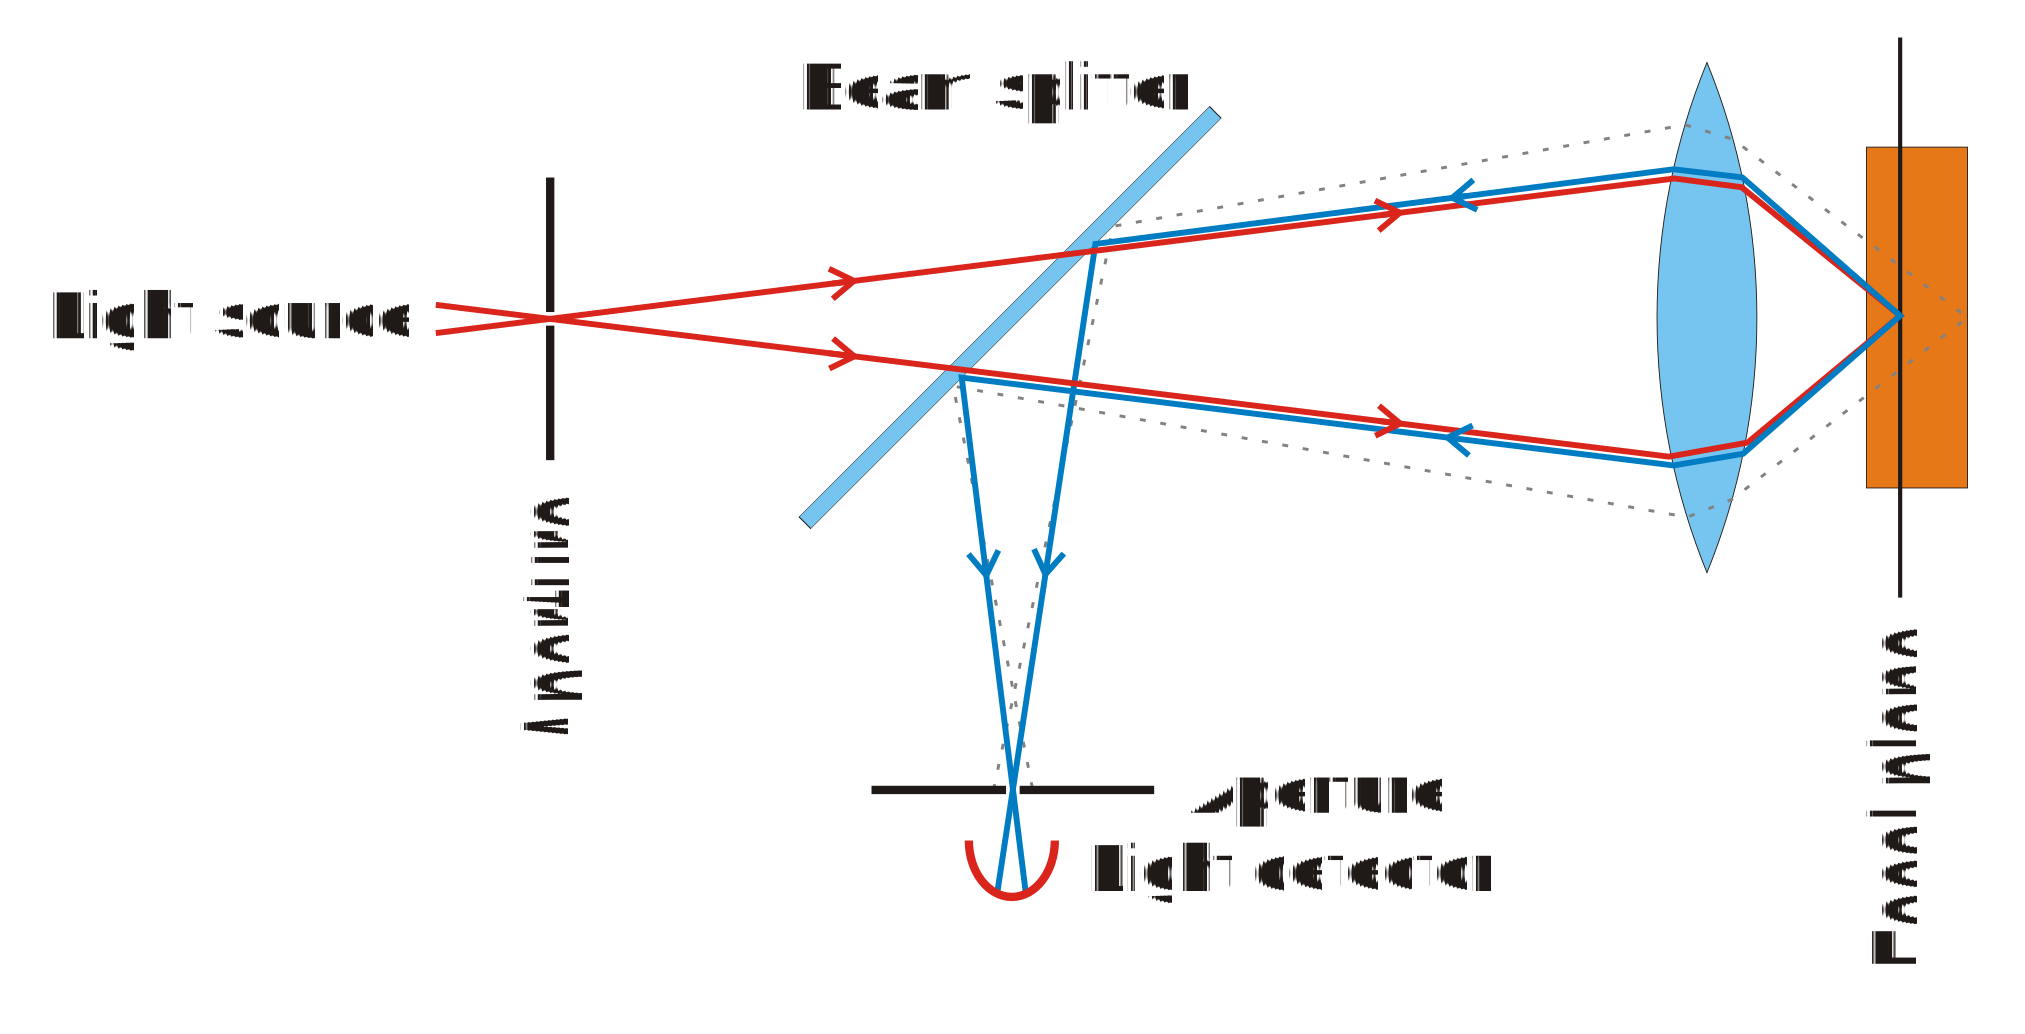
\includegraphics[width=0.95\textwidth]{pictures/ConfocalPrinciple}
%\end{center}
%\caption{Confocal microscope principle (source:\href{http://en.wikipedia.org/wiki/File:Confocalprinciple.svg}{Wikipedia})}
%\label{fig:ConfocalPrinciple}
%\end{figure}
%
%\begin{figure}[htb]
%\begin{center}
%\leavevmode
% 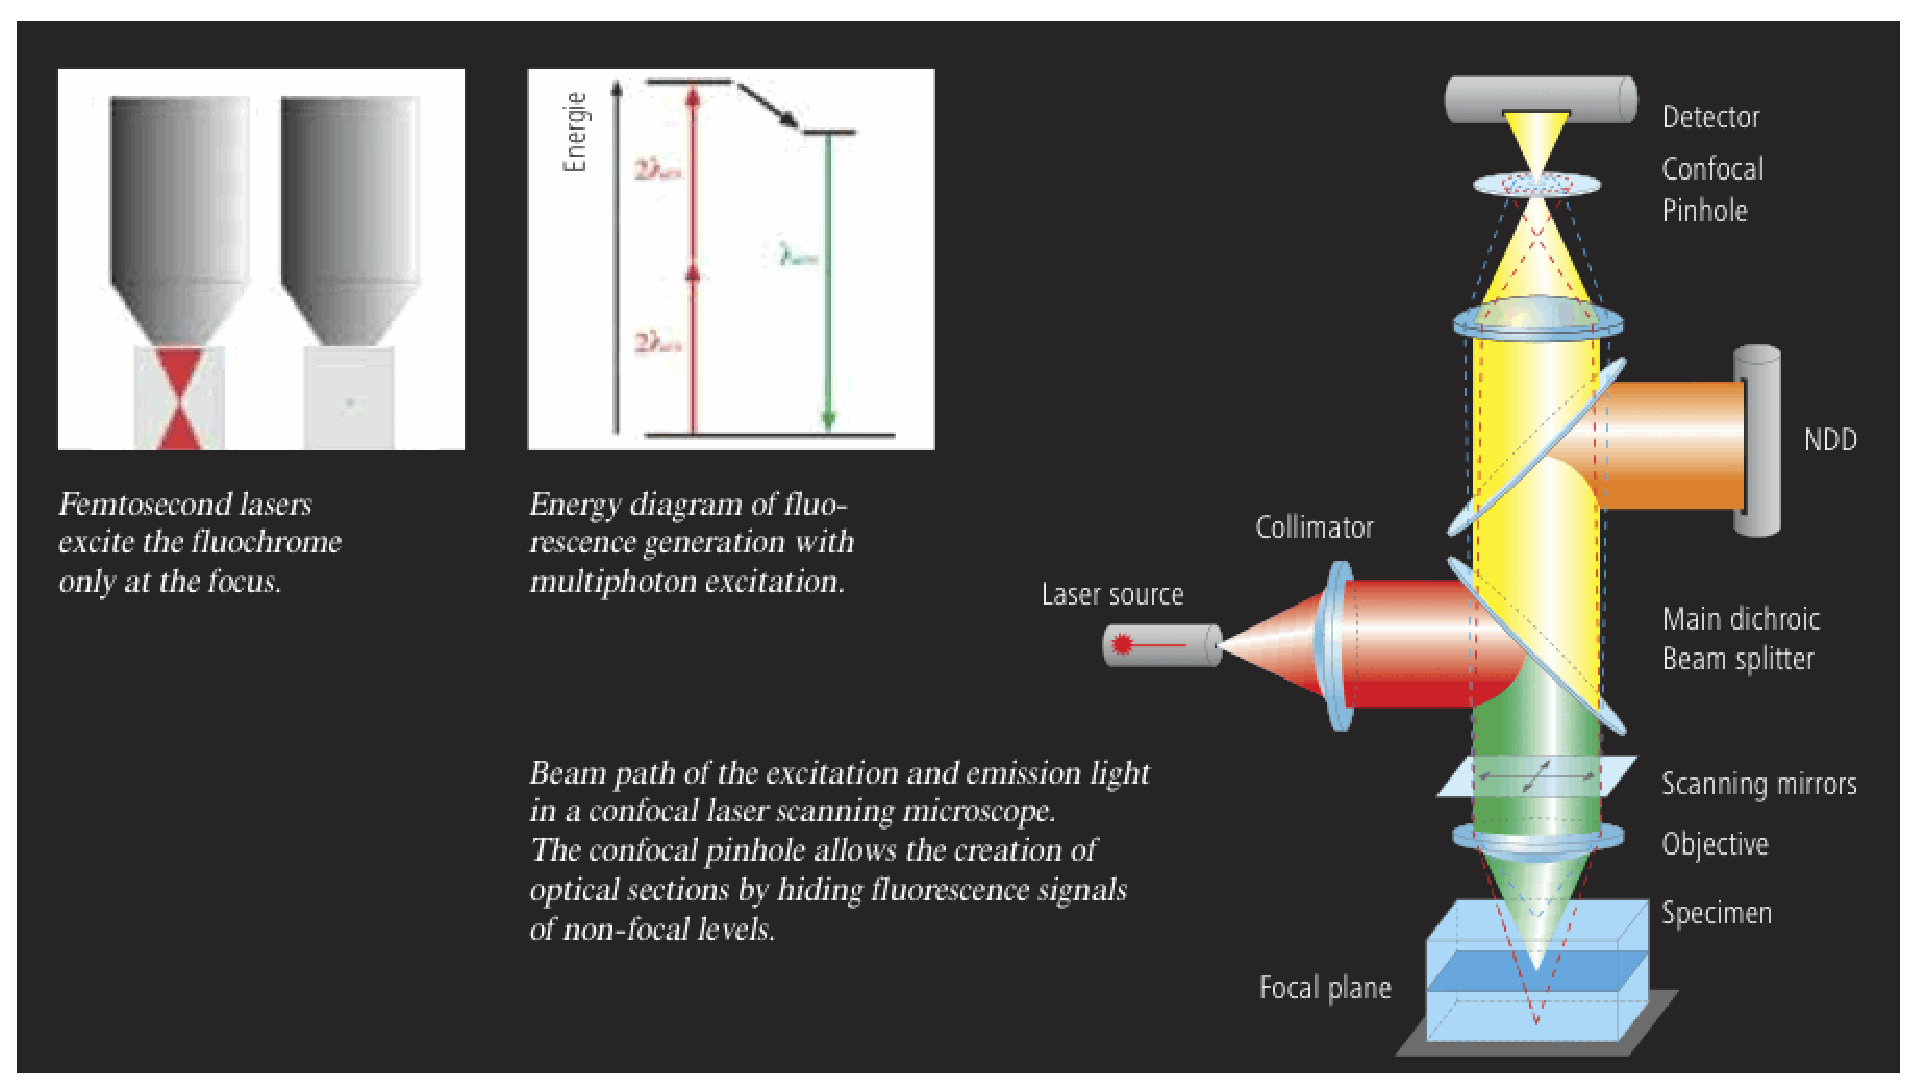
\includegraphics[width=0.95\textwidth]{pictures/ConfocalZeissPrinciple}
%\end{center}
%\caption{2-photon confocal microscope principle (Zeiss documentation)}
%\label{fig:Confocal2photonsPrinciple}
%\end{figure}
%
%\begin{figure}[htb]
%\begin{center}
%\leavevmode
%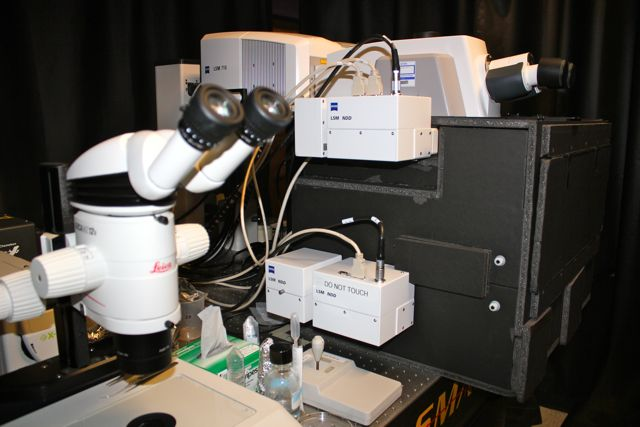
\includegraphics[width=0.95\textwidth]{pictures/PICmicroscope}
%\end{center}
%\caption{2-photon confocal microscope Zeiss 710 NLO in service in the Megason Lab}
%\label{fig:MicMegason}
%\end{figure}


\section{Problematic}


As discussed previously, membrane segmentation is an important step in the process of understanding the development of an embryo.
Indeed, membrane provide useful informations on the local connectivity between cells, and on local characteristics of a given cell (like volume, shape information...).
Segmenting cell membrane is a challenging problem (see section~\ref{}): data are incomplete, quite noisy, 3D and anisotropic.

Due to the physics of the image acquisition, data are never complete and thus any segmentation technique need serious prior to properly extract cell membrane.
An assumption based on biological knowledge is that each nucleus belongs to one cell, and is inside the space enclosed by the cell membrane.
Two important points should be pointed out from this assumption:
\begin{itemize}
    \item cell membranes are closed
    \item cell nuclei center are inside
\end{itemize}

Under this assumption, correctly detecting nuclei is thus really important to extract cell membrane in images.
In my thesis, I will focus on cell nuclei detection in order to efficiently extract and segment cell membranes.
In the rest of the document, I shall first present the data to be processed, and existing method for nuclei segmentation;
then, I will introduce my technique in which I make use of information from the nuclei channel and the membrane channel;
I will present results of my method on synthetic data sets, as well as on real data sets, with validation and comparison with existing methods.
Finally, I will conclude and suggest some improvements to my method and some future plans in order to use this method for segmenting cell membranes. 
